% Provenance (never printed): BCPST year 1 geology (2021), "la carte
% geologique" (reading a map, structures, chronology), union licence
% Sciences de la Terre L1 (cartographie: strike and dip, three-point problem,
% outcrop patterns, DEM and GIS). See sources/outline_sources.md. Pilot
% chapter, 2026-10-22. The region is the series' invented Varden Hills
% (figdata/shared/region.py); every number about it is computed in
% figdata/bachelor-1/varden_maps.py or figdata/bachelor-1/v_rule.py.
\chapter{Geological Maps}\label{ch:b1:geological-maps}

A geologist crosses a range of low hills with a map board, a notebook and a
compass-clinometer. Most of the ground is grass, wood or ploughed field; rock
shows only here and there, in a stream bank, a road cutting, a crag. From these
scattered glimpses, and from the shape of the land, the geologist must say which rock
lies under every square metre of the hills, how the layers are tilted, where
they are broken, and in what order all this happened. The result is a
\omterm{def:b1:geological-maps:geological-map}{geological map}: a flat drawing that encodes a three-dimensional body of rock.
This chapter explains how such a map is made and how it is read --- how the
\omterm{def:b1:geological-maps:attitude}{attitude} of a surface is measured and computed, why the \omterm{def:b1:geological-maps:geological-map}{outcrop} of a layer
draws the patterns it does, and how a map tells a history. Its examples come
from an imaginary but geologically consistent region, the Varden Hills, which
recurs throughout this book.

\begin{recall}
A topographic map shows the relief with contour lines, lines of equal
elevation; its scale relates distances on the map to distances on the ground
(Book 1, grade 9). Relative ages follow from superposition (a layer is
younger than the layers below it, unless the sequence has been overturned),
from cross-cutting (whatever cuts a rock is younger than it) and from
inclusion (Book 1, grade 7). A fault is a fracture along which the two blocks
have moved (Book 1, grade 7); the geometry of \omterm{def:b1:geological-maps:fold}{folds} and faults is the subject
of \cref{ch:b1:faults-folds-fabrics}.
\end{recall}

\section{A map is a cut through three dimensions}\label{sec:b1:geological-maps:cut}

\begin{definition}[Geological map]\label{def:b1:geological-maps:geological-map}
A \emph{geological map}\index{geological map} shows, at every point of the
ground surface, the rock unit that lies there beneath the soil, with the
\emph{contacts}\index{contact (geological)} --- the surfaces separating two
units --- and the structures (faults, \omterm{def:b1:geological-maps:fold}{fold} axes, \omterm{def:b1:geological-maps:attitude}{attitudes} of layers) that
affect them. A \emph{map unit}\index{map unit} is a body of rock that can be
recognised and followed in the field and is drawn in one colour; its
\emph{outcrop}\index{outcrop} is the area where it lies at the surface.
\end{definition}

\begin{definition}[Digital elevation model]\label{def:b1:geological-maps:dem}
A \emph{digital elevation model}\index{digital elevation model} is a grid of
ground elevations, $z = g(x,y)$, at regularly spaced points. A geographic
information system stores such grids and the map's other layers (\omterm{def:b1:geological-maps:geological-map}{contacts},
faults, measurements, boreholes) in a common frame of coordinates and
computes with them.
\end{definition}

\begin{proposition}[The outcrop of a contact]\label{prop:b1:geological-maps:intersection}
Let the ground be the surface $z = g(x,y)$ and a contact the surface
$z = c(x,y)$. The trace of the contact on the map is the curve
\[
  g(x,y) = c(x,y),
\]
the projection on the horizontal plane of the intersection of the two
surfaces. The unit lying above the contact crops out where $g > c$.
\end{proposition}

\begin{proof}
A point of the map lies on the trace if and only if the ground surface at
that point belongs to the contact, that is $g(x,y) = c(x,y)$. Where
$g(x,y) > c(x,y)$, the ground is above the contact: the rock at the surface
belongs to the unit lying above it.
\end{proof}

\begin{remark}[How the maps of this book are drawn]\label{rem:b1:geological-maps:computed}
This is exactly how a geographic information system draws a map from a
three-dimensional model: it evaluates $g - c$ on the grid of a \omterm{def:b1:geological-maps:dem}{digital
elevation model} and traces the curves where it changes sign. The maps of
the Varden Hills in this book were drawn that way, from a geological model
in which every surface is known.
\end{remark}

\begin{omfigure}
\begin{tikzpicture}
\begin{axis}[axis equal image, xmin=0, xmax=10, ymin=0, ymax=8, width=0.82\linewidth,
  tick label style={font=\scriptsize}, xlabel={east (km)}, ylabel={north (km)},
  label style={font=\small}, colormap/blackwhite, enlargelimits=false]
\addplot[matrix plot*, mesh/cols=101, point meta=explicit, shader=interp] table[x=x_km, y=y_km, meta=shade] {figdata/out/bachelor-1-varden_maps-shade.dat};
\addplot[contour, line width=0.25pt, opacity=0.7] table {figdata/out/shared-region-contours.dat};
\addplot[index contour, opacity=0.8] table {figdata/out/shared-region-index-contours.dat};
\addplot[river] table {figdata/out/shared-region-river.dat};
\end{axis}
\end{tikzpicture}

{\small The Varden Hills as a \omterm{def:b1:geological-maps:dem}{digital elevation model}: the ground lit from
the north-west, with contours every \qty{50}{m} (thicker at 250 and
\qty{500}{m}) and the river, which flows east.}
\end{omfigure}

\begin{omfigure}
\begin{tikzpicture}
\begin{axis}[axis equal image, xmin=0, xmax=10, ymin=0, ymax=8, width=0.82\linewidth,
  tick label style={font=\scriptsize}, xlabel={east (km)}, ylabel={north (km)},
  label style={font=\small}]
\addplot[lith schist, draw=black, line width=0.3pt, even odd rule] table {figdata/out/shared-region-unit-schist.dat};
\addplot[lith granite, draw=black, line width=0.3pt, even odd rule] table {figdata/out/shared-region-unit-granite.dat};
\addplot[om lith={icsTriassic!35}{om sand}, draw=black, line width=0.3pt, even odd rule] table {figdata/out/shared-region-unit-sandstone.dat};
\addplot[om lith={icsJurassic!40}{om limestone}, draw=black, line width=0.3pt, even odd rule] table {figdata/out/shared-region-unit-limestone.dat};
\addplot[om lith={icsJurassic!15}{om shale}, draw=black, line width=0.3pt, even odd rule] table {figdata/out/shared-region-unit-shale.dat};
\addplot[om lith={icsCretaceous!35}{om limestone}, draw=black, line width=0.3pt, even odd rule] table {figdata/out/shared-region-unit-chalk.dat};
% the fault is drawn before the alluvium: the younger alluvial floor conceals it
\addplot[normal fault] table {figdata/out/shared-region-fault.dat};
\addplot[lith alluvium, draw=black, line width=0.3pt, even odd rule] table {figdata/out/shared-region-unit-alluvium.dat};
\addplot[contour, opacity=0.55] table {figdata/out/shared-region-contours.dat};
\addplot[river] table {figdata/out/shared-region-river.dat};
\pic at (axis cs:4.3,6.6) {strikedip={350.6}{12}};
\pic at (axis cs:2.2,6.6) {strikedip={189.3}{12}};
\pic at (axis cs:8.6,1.4) {northarrow};
\fill[black] (axis cs:6.6,0.35) rectangle (axis cs:7.1,0.5);
\fill[white] (axis cs:7.1,0.35) rectangle (axis cs:7.6,0.5);
\fill[black] (axis cs:7.6,0.35) rectangle (axis cs:8.1,0.5);
\fill[white] (axis cs:8.1,0.35) rectangle (axis cs:8.6,0.5);
\draw[black, line width=0.4pt] (axis cs:6.6,0.35) rectangle (axis cs:8.6,0.5);
\node[font=\footnotesize, above, inner sep=1.5pt, fill=white, fill opacity=0.8, text opacity=1] at (axis cs:7.6,0.5) {\qty{2}{km}};
\end{axis}
\end{tikzpicture}

\smallskip
\begin{tikzpicture}[font=\footnotesize]
\matrix[column sep=7pt, row sep=3pt, matrix of nodes, nodes={anchor=west}] {
  \tikz\draw[black!60, line width=0.4pt, lith alluvium] (0,0) rectangle (0.7,0.32); & alluvium (Quaternary) &
  \tikz\draw[black!60, line width=0.4pt, om lith={icsCretaceous!35}{om limestone}] (0,0) rectangle (0.7,0.32); & chalk (Cretaceous, 90 Ma) \\
  \tikz\draw[black!60, line width=0.4pt, om lith={icsJurassic!15}{om shale}] (0,0) rectangle (0.7,0.32); & shale (Jurassic, 165 Ma) &
  \tikz\draw[black!60, line width=0.4pt, om lith={icsJurassic!40}{om limestone}] (0,0) rectangle (0.7,0.32); & limestone (Jurassic, 180 Ma) \\
  \tikz\draw[black!60, line width=0.4pt, om lith={icsTriassic!35}{om sand}] (0,0) rectangle (0.7,0.32); & sandstone (Triassic, 245 Ma) &
  \tikz\draw[black!60, line width=0.4pt, lith granite] (0,0) rectangle (0.7,0.32); & granite (310 Ma) \\
  \tikz\draw[black!60, line width=0.4pt, lith schist] (0,0) rectangle (0.7,0.32); & schist (480 Ma) &
  \tikz\draw[normal fault] (0,0.16) -- (0.9,0.16); & normal fault (ticks on the downthrown side) \\
};
\end{tikzpicture}

{\small The \omterm{def:b1:geological-maps:geological-map}{geological map} of the Varden Hills, with the contours, the river,
two measured \omterm{def:b1:geological-maps:attitude}{attitudes} (\omterm{def:b1:geological-maps:attitude}{strike} line and \omterm{def:b1:geological-maps:attitude}{dip} tick, with the \omterm{def:b1:geological-maps:attitude}{dip} in degrees)
and the legend. The ages are those of the region's units; the fault is
hidden beneath the younger alluvium of the valley floor.}
\end{omfigure}

\section{The attitude of a plane}

\begin{definition}[Strike, dip and dip direction]\label{def:b1:geological-maps:attitude}
Let a geological surface --- a bedding plane, a contact, a fault --- be
locally a plane. Its \emph{strike}\index{strike} is the direction of the
horizontal lines it contains, given as an \omterm{def:b1:spherical-astronomy:horizontal}{azimuth} (degrees clockwise from
north). Its \emph{dip}\index{dip} $\delta$ is the angle between the plane and
the horizontal, measured in the vertical plane perpendicular to the strike,
$0 \le \delta \le \ang{90}$. Its \emph{dip direction}\index{dip direction}
$\alpha$ is the \omterm{def:b1:spherical-astronomy:horizontal}{azimuth} of the steepest downward line of the plane. Together
they form the plane's \emph{attitude}\index{attitude (of a plane)}, written
dip direction/dip, for instance $080/12$.
\end{definition}

\begin{notation}[Strike by the right-hand rule]\label{not:b1:geological-maps:rhr}
A \omterm{def:b1:geological-maps:attitude}{strike} can be read in two opposite directions. The \emph{right-hand rule}
chooses the one for which the plane \omterm{def:b1:geological-maps:attitude}{dips} to the right of an observer looking
along the \omterm{def:b1:geological-maps:attitude}{strike}: \omterm{def:b1:geological-maps:attitude}{strike} $= \alpha - \ang{90}$ (modulo \ang{360}). On a map,
the symbol is a \omterm{def:b1:geological-maps:attitude}{strike} line with a short tick pointing down the \omterm{def:b1:geological-maps:attitude}{dip}, labelled
with the \omterm{def:b1:geological-maps:attitude}{dip}.
\end{notation}

\begin{omfigure}
\tdplotsetmaincoords{65}{125}
\begin{tikzpicture}[tdplot_main_coords, font=\small, scale=1.05]
  % the horizontal plane
  \fill[omSea!50] (-2.2,-1.6,0) -- (2.2,-1.6,0) -- (2.2,1.6,0) -- (-2.2,1.6,0) -- cycle;
  \draw[black!40] (-2.2,-1.6,0) -- (2.2,-1.6,0) -- (2.2,1.6,0) -- (-2.2,1.6,0) -- cycle;
  % the dipping plane: strike along y (north), dipping east (+x) at 30 degrees
  \fill[omLithLime!80, opacity=0.85] (-0.0,-1.6,0) -- (-0.0,1.6,0) -- (2.2,1.6,-1.27) -- (2.2,-1.6,-1.27) -- cycle;
  \draw[black!60] (0,-1.6,0) -- (0,1.6,0) -- (2.2,1.6,-1.27) -- (2.2,-1.6,-1.27) -- cycle;
  % strike line (horizontal, in both planes)
  \draw[omThm, line width=1.1pt] (0,-1.6,0) -- (0,1.6,0);
  % dip line and the horizontal below it, with the dip angle
  \draw[omDef, line width=1.1pt, -{Stealth[length=2.4mm]}] (0,0,0) -- (2.2,0,-1.27);
  \draw[black!60, densely dashed] (0,0,0) -- (2.2,0,0);
  \draw[black!60, densely dashed] (2.2,0,0) -- (2.2,0,-1.27);
  \draw[black] plot[domain=0:30, samples=16, variable=\t] ({0.8*cos(\t)}, 0, {-0.8*sin(\t)});
  \node[font=\footnotesize] at (1.05,0,-0.22) {$\delta$};
  % north arrow on the horizontal plane
  \draw[black, -{Stealth[length=2mm]}] (-1.8,-1.2,0) -- (-1.8,-0.3,0);
  \node[font=\footnotesize] at (-1.8,-0.05,0) {N};
\end{tikzpicture}
\begin{tikzpicture}[font=\small]
  \node[align=left, anchor=west, text width=5.2cm] at (0,0) {%
    \textcolor{omThm}{\rule[0.5ex]{0.6cm}{1.1pt}} strike: a horizontal line of the plane;\\[3pt]
    \textcolor{omDef}{\rule[0.5ex]{0.6cm}{1.1pt}} the steepest line down the plane, whose azimuth is the dip direction;\\[3pt]
    the dip is the angle between this line and the horizontal (dashed).};
\end{tikzpicture}

{\small A plane striking north and dipping \ang{30} to the east (\omterm{def:b1:geological-maps:attitude}{attitude}
$090/30$), cutting a horizontal plane along its \omterm{def:b1:geological-maps:attitude}{strike} line. Not to scale.}
\end{omfigure}

\begin{proposition}[The equation of a dipping plane]\label{prop:b1:geological-maps:plane}
With $x$ to the east, $y$ to the north and $z$ upward, the plane of \omterm{def:b1:geological-maps:attitude}{dip
direction} $\alpha$ and \omterm{def:b1:geological-maps:attitude}{dip} $\delta$ through the point $(x_0, y_0, z_0)$ is
\[
  z = z_0 - \tan\delta\,\bigl[(x - x_0)\sin\alpha + (y - y_0)\cos\alpha\bigr].
\]
\end{proposition}

\begin{proof}
The horizontal unit vector pointing in the \omterm{def:b1:geological-maps:attitude}{dip direction} is
$\vec u = (\sin\alpha, \cos\alpha, 0)$ (an \omterm{def:b1:spherical-astronomy:horizontal}{azimuth} is measured from north,
the $y$ axis, toward east, the $x$ axis). Along the \omterm{def:b1:geological-maps:attitude}{strike}, perpendicular to
$\vec u$, the plane is horizontal; along $\vec u$ it descends by
$\tan\delta$ per unit of horizontal distance. The horizontal distance of a
point from the \omterm{def:b1:geological-maps:attitude}{strike} line through $(x_0, y_0)$, counted positive \omterm{def:b1:geological-maps:attitude}{down-dip},
is $(x-x_0)\sin\alpha + (y-y_0)\cos\alpha$, whence the formula.
\end{proof}

\begin{theorem}[Attitude from three points]\label{thm:b1:geological-maps:three-point}
Let $P_1, P_2, P_3$ be three non-collinear points of a plane, and
$\vec n = \overrightarrow{P_1P_2} \times \overrightarrow{P_1P_3} =
(n_x, n_y, n_z)$, chosen with $n_z > 0$ (replace $\vec n$ by $-\vec n$
otherwise). Then the \omterm{def:b1:geological-maps:attitude}{dip} and the \omterm{def:b1:geological-maps:attitude}{dip direction} of the plane are
\[
  \delta = \arccos\frac{n_z}{\|\vec n\|}, \qquad
  \alpha = \text{the azimuth of the horizontal vector } (n_x, n_y),
\]
that is the angle $\alpha \in [\ang{0}, \ang{360})$ with
$\sin\alpha = n_x/\sqrt{n_x^2+n_y^2}$ and $\cos\alpha = n_y/\sqrt{n_x^2+n_y^2}$
(the plane is horizontal if $n_x = n_y = 0$).
\end{theorem}

\begin{proof}
$\vec n$ is perpendicular to two independent vectors of the plane, hence
normal to it. The \omterm{def:b1:geological-maps:attitude}{dip} is the angle between the plane and the horizontal,
equal to the angle between their normals, $\vec n$ and the vertical
$\vec k$: $\cos\delta = \vec n \cdot \vec k / \|\vec n\| = n_z/\|\vec n\|$.
By \cref{prop:b1:geological-maps:plane}, the plane is $z = \text{const} -
\tan\delta\,(x\sin\alpha + y\cos\alpha)$, that is
$\tan\delta\sin\alpha\,x + \tan\delta\cos\alpha\,y + z = \text{const}$; its
upward normal is proportional to $(\tan\delta\sin\alpha,
\tan\delta\cos\alpha, 1)$, whose horizontal part points in the \omterm{def:b1:geological-maps:attitude}{dip direction}
$\alpha$. Since $\vec n$ is a positive multiple of this normal, $(n_x, n_y)$
points in the \omterm{def:b1:geological-maps:attitude}{dip direction} too.
\end{proof}

\begin{method}[The three-point problem]\label{met:b1:geological-maps:three-point}
To find the \omterm{def:b1:geological-maps:attitude}{attitude} of a contact met in three boreholes (or seen at three
\omterm{def:b1:geological-maps:geological-map}{outcrops}):
\begin{enumerate}
  \item for each borehole, take the elevation of the contact: the ground
        elevation minus the depth at which the contact was met;
  \item write the three points $P_i = (x_i, y_i, z_i)$ in metres, $x$ east,
        $y$ north;
  \item compute $\vec n = \overrightarrow{P_1P_2} \times
        \overrightarrow{P_1P_3}$ and make $n_z$ positive;
  \item apply \cref{thm:b1:geological-maps:three-point}; give the \omterm{def:b1:geological-maps:attitude}{attitude}
        as \omterm{def:b1:geological-maps:attitude}{dip direction}/\omterm{def:b1:geological-maps:attitude}{dip} and, if asked, the \omterm{def:b1:geological-maps:attitude}{strike} by the right-hand
        rule.
\end{enumerate}
On paper, the same problem is solved with structure contours: on the line
joining the highest and the lowest point, find by proportion the point at
the elevation of the third one; the line through these two points of equal
elevation is a \omterm{def:b1:geological-maps:attitude}{strike} line; the \omterm{def:b1:geological-maps:attitude}{dip} follows from the elevation difference
between two parallel \omterm{def:b1:geological-maps:attitude}{strike} lines and their spacing.
\end{method}

\begin{example}[The east limb of the Varden anticline]\label{ex:b1:geological-maps:east}
% computed in figdata/bachelor-1/varden_maps.py (boreholes E1-E3)
Three boreholes, E1 at $(4000, 6000)$, E2 at $(4600, 7200)$ and E3 at
$(5100, 6400)$ (metres east and north of the map's south-west corner), meet
the base of the limestone at elevations $174$, $4$ and $\qty{-74}{m}$. Then
$\overrightarrow{P_1P_2} = (600, 1200, -170)$,
$\overrightarrow{P_1P_3} = (1100, 400, -248)$; their cross product is
$(-229\,600, -38\,200, -1\,080\,000)$, which points downward, so
\[
  \vec n = (229\,600,\ 38\,200,\ 1\,080\,000).
\]
Hence $\cos\delta = 1\,080\,000/\|\vec n\| \approx
0.9776$, $\delta \approx \ang{12.2}$, and the \omterm{def:b1:geological-maps:attitude}{dip direction} is the \omterm{def:b1:spherical-astronomy:horizontal}{azimuth} of
$(229\,600, 38\,200)$, $\alpha \approx \ang{80.6}$: the \omterm{def:b1:geological-maps:attitude}{attitude} is
$081/12$, \omterm{def:b1:geological-maps:attitude}{strike} $\ang{351}$ by the right-hand rule. The base of the
limestone \omterm{def:b1:geological-maps:attitude}{dips} gently east-north-east.
\end{example}

\section{Outcrop patterns}

\begin{proposition}[Horizontal and vertical contacts]\label{prop:b1:geological-maps:hv}
The trace of a horizontal contact follows the contour line of its elevation.
The trace of a vertical contact is a straight line on the map, whatever the
relief.
\end{proposition}

\begin{proof}
For $c(x,y) = z_0$, the trace $g(x,y) = z_0$ is the contour $z_0$
(\cref{prop:b1:geological-maps:intersection}). A vertical plane is the set of
points whose horizontal position lies on one straight line, at any elevation;
its trace on the map is that line.
\end{proof}

\begin{theorem}[The V-rule]\label{thm:b1:geological-maps:v-rule}
A planar contact crosses a valley whose floor descends downstream with
gradient $s > 0$. Let $a$ be the tangent of the contact's apparent \omterm{def:b1:geological-maps:attitude}{dip} in
the downstream direction ($a > 0$ if it \omterm{def:b1:geological-maps:attitude}{dips} downstream, $a < 0$ if it \omterm{def:b1:geological-maps:attitude}{dips}
upstream, $a = 0$ if horizontal). Then the \omterm{def:b1:geological-maps:geological-map}{outcrop} trace makes a V whose apex
lies on the valley floor and
\begin{itemize}
  \item points \emph{downstream} if $a > s$: the contact \omterm{def:b1:geological-maps:attitude}{dips} downstream more
        steeply than the valley floor descends;
  \item points \emph{upstream} if $a < s$: the contact is horizontal, \omterm{def:b1:geological-maps:attitude}{dips}
        upstream, or \omterm{def:b1:geological-maps:attitude}{dips} downstream less steeply than the floor.
\end{itemize}
A vertical contact makes no V.
\end{theorem}

\begin{proof}
Let $\xi$ be the distance measured downstream along the valley floor. The
floor is at elevation $z_g(\xi) = z_0 - s\xi$; in the vertical section
along the valley, the contact is at $z_c(\xi) = c - a\xi$. On the floor the
trace is where $z_g = z_c$:
\[
  \xi_{\text{floor}} = \frac{c - z_0}{a - s}.
\]
On a valley side, at a point higher than the floor by $h > 0$ and at the
same distance from the valley's source, the ground is at $z_0 - s\xi + h$, so
the trace is where $c - a\xi = z_0 - s\xi + h$:
\[
  \xi_{\text{side}} = \frac{c - z_0 - h}{a - s}, \qquad
  \xi_{\text{floor}} - \xi_{\text{side}} = \frac{h}{a - s}.
\]
If $a > s$, the trace lies farther downstream on the floor than on the
sides: the V points downstream. If $a < s$, the reverse. A vertical contact
crosses the floor and the sides at the same $\xi$.
\end{proof}

\begin{omfigure}
\begin{tikzpicture}
\pgfplotsset{vpanel/.style={axis equal image, xmin=-1, xmax=1, ymin=0, ymax=2,
  width=4.1cm, ticks=none, axis line style={black!50}, clip=true,
  title style={font=\footnotesize, align=center, yshift=-2pt}}}
\begin{axis}[vpanel, at={(0cm,0cm)}, title={horizontal}]
\addplot[contour, opacity=0.8] table {figdata/out/bachelor-1-v_rule-contours.dat};
\addplot[omThm, line width=1.2pt] table {figdata/out/bachelor-1-v_rule-h.dat};
\addplot[river, -{Stealth[length=1.6mm]}] coordinates {(0,0.05) (0,1.95)};
\end{axis}
\begin{axis}[vpanel, at={(3.15cm,0cm)}, title={dipping\\upstream}]
\addplot[contour, opacity=0.8] table {figdata/out/bachelor-1-v_rule-contours.dat};
\addplot[omThm, line width=1.2pt] table {figdata/out/bachelor-1-v_rule-u.dat};
\addplot[river, -{Stealth[length=1.6mm]}] coordinates {(0,0.05) (0,1.95)};
\end{axis}
\begin{axis}[vpanel, at={(6.3cm,0cm)}, title={downstream,\\gentler than floor}]
\addplot[contour, opacity=0.8] table {figdata/out/bachelor-1-v_rule-contours.dat};
\addplot[omThm, line width=1.2pt] table {figdata/out/bachelor-1-v_rule-g.dat};
\addplot[river, -{Stealth[length=1.6mm]}] coordinates {(0,0.05) (0,1.95)};
\end{axis}
\begin{axis}[vpanel, at={(9.45cm,0cm)}, title={downstream,\\steeper than floor}]
\addplot[contour, opacity=0.8] table {figdata/out/bachelor-1-v_rule-contours.dat};
\addplot[omThm, line width=1.2pt] table {figdata/out/bachelor-1-v_rule-d.dat};
\addplot[river, -{Stealth[length=1.6mm]}] coordinates {(0,0.05) (0,1.95)};
\end{axis}
\end{tikzpicture}

{\small The V-rule computed. In each panel a river (blue arrow) flows north
down a valley, whose contours (every \qty{10}{m}) point upstream; a contact
striking east--west is traced in red. Horizontal, it follows the contours;
dipping upstream, or downstream less steeply than the valley floor, it makes
a V pointing upstream; dipping downstream more steeply (here \ang{10}), a V
pointing downstream. A vertical contact would cross straight.}
\end{omfigure}

\begin{remark}[The width of an outcrop]\label{rem:b1:geological-maps:width}
The width of a unit's \omterm{def:b1:geological-maps:geological-map}{outcrop} depends on its thickness, on its \omterm{def:b1:geological-maps:attitude}{dip} and on the
slope of the ground: a thin layer dipping in the same direction as the slope
can crop out over a wide area. Thickness is computed from a map and a
cross-section in \cref{ch:b1:cross-sections}.
\end{remark}

\section{Folds, faults, intrusions and unconformities on a map}

\begin{definition}[Anticline and syncline]\label{def:b1:geological-maps:fold}
A \emph{fold}\index{fold} is a bend of once-planar layers. An
\emph{anticline}\index{anticline} is a fold whose layers are convex upward
(an upfold); a \emph{syncline}\index{syncline} is a fold whose layers are
concave upward (a downfold). The two sides of a fold are its limbs; its
\emph{fold axis}\index{fold axis} is the line along which the layers bend
most, and the axis plunges when it is not horizontal. A line such as a fold
axis is located by its trend, the \omterm{def:b1:spherical-astronomy:horizontal}{azimuth} of its horizontal projection taken
in the downward direction, and its plunge, the angle it makes with the
horizontal (\cref{ch:b1:field-lab-methods-1}). Fold geometry in
three dimensions is the subject of \cref{ch:b1:faults-folds-fabrics}.
\end{definition}

\begin{proposition}[Fold patterns]\label{prop:b1:geological-maps:folds}
On a map of eroded folded layers, an \omterm{def:b1:geological-maps:fold}{anticline} shows the oldest
units in its core and younger units outward on both sides; a \omterm{def:b1:geological-maps:fold}{syncline}
shows the youngest in its core. If the \omterm{def:b1:geological-maps:fold}{fold axis} plunges, the
\omterm{def:b1:geological-maps:geological-map}{outcrops} close around the \omterm{def:b1:geological-maps:fold}{fold}: the closure of an \omterm{def:b1:geological-maps:fold}{anticline} points in the
direction of plunge, that of a \omterm{def:b1:geological-maps:fold}{syncline} the opposite way.
\end{proposition}

\begin{proof}[Partial proof]
In an \omterm{def:b1:geological-maps:fold}{anticline} the layers rise toward the axis, so a roughly level erosion
surface cuts deepest into the sequence there and exposes its oldest, lowest
units; in a \omterm{def:b1:geological-maps:fold}{syncline} the youngest units are preserved lowest, in the core. If
the axis plunges, consider a contact of an \omterm{def:b1:geological-maps:fold}{anticline}: it is an arch whose
crest descends along the plunge. Where the crest is above the ground, the
ground cuts the arch along two limbs; where the crest passes below the
ground, the contact no longer reaches the surface. The two limbs of the trace
therefore join round the point where the crest meets the ground, and that
closure lies in the direction of plunge. A \omterm{def:b1:geological-maps:fold}{syncline} is a trough whose bottom
rises the opposite way, so its closure points against the plunge. The
argument assumes gentle relief compared with the drop of the axis.
\end{proof}

\begin{proposition}[Faults, intrusions and unconformities]\label{prop:b1:geological-maps:cuts}
On a map:
\begin{itemize}
  \item a fault interrupts and offsets the \omterm{def:b1:geological-maps:geological-map}{contacts} it crosses; on the block
        that moved down, younger units come to the surface opposite older
        ones; the trace of a dipping fault obeys the V-rule like any plane;
  \item a pluton or a dyke cuts across the \omterm{def:b1:geological-maps:geological-map}{contacts} of the rocks it intrudes,
        and is younger than them;
  \item at an unconformity, the \omterm{def:b1:geological-maps:geological-map}{contacts} of the older rocks are cut off
        along the base of the younger ones, which may rest on several older
        units in turn.
\end{itemize}
\end{proposition}

\begin{method}[Reading the history from a map]\label{met:b1:geological-maps:history}
\begin{enumerate}
  \item List the units in order of age, from the legend and from
        superposition.
  \item Find what cuts what: faults, intrusions, unconformities; each is
        younger than everything it cuts and older than everything that seals
        it.
  \item Find the \omterm{def:b1:geological-maps:fold}{folds} and their axes; a \omterm{def:b1:geological-maps:fold}{fold} is younger than the youngest
        unit it \omterm{def:b1:geological-maps:fold}{folds}.
  \item Write the events in order, each with the evidence on the map.
\end{enumerate}
\end{method}

\begin{example}[The history of the Varden Hills]\label{ex:b1:geological-maps:history}
On the map of the Varden Hills: the schist is the oldest unit; the granite
cuts it, so it is younger; the sandstone rests on both, cutting off the
granite's outline: an unconformity, after a long erosion. The sandstone,
limestone, shale and chalk follow one another without a break and are folded
together into an \omterm{def:b1:geological-maps:fold}{anticline} (sandstone and basement in the core, near
$x = \qty{3.5}{km}$) and a \omterm{def:b1:geological-maps:fold}{syncline} (chalk in the core, east of the map's
centre): the folding came after the chalk was laid down. The fault offsets
the folded \omterm{def:b1:geological-maps:geological-map}{contacts}: it is younger than the folding. Finally the river has
cut down and spread its alluvium, which no fault breaks.
\end{example}

\begin{inthefield}[Measuring an attitude]
On a clean bedding surface, the geologist lays the edge of a
compass-clinometer horizontal and reads the \omterm{def:b1:geological-maps:attitude}{strike} on the compass, then sets
it down the steepest slope and reads the \omterm{def:b1:geological-maps:attitude}{dip} on the clinometer. Every
measurement is written in the notebook with its position and plotted on the
map at once, so that an inconsistent reading shows up while the \omterm{def:b1:geological-maps:geological-map}{outcrop} is
still at hand. Today, positions come from satellite receivers, measurements
are entered on tablets that run a geographic information system, and
\omterm{def:b1:geological-maps:geological-map}{outcrops} are photographed and placed on \omterm{def:b1:geological-maps:dem}{digital elevation models}.
\begin{center}
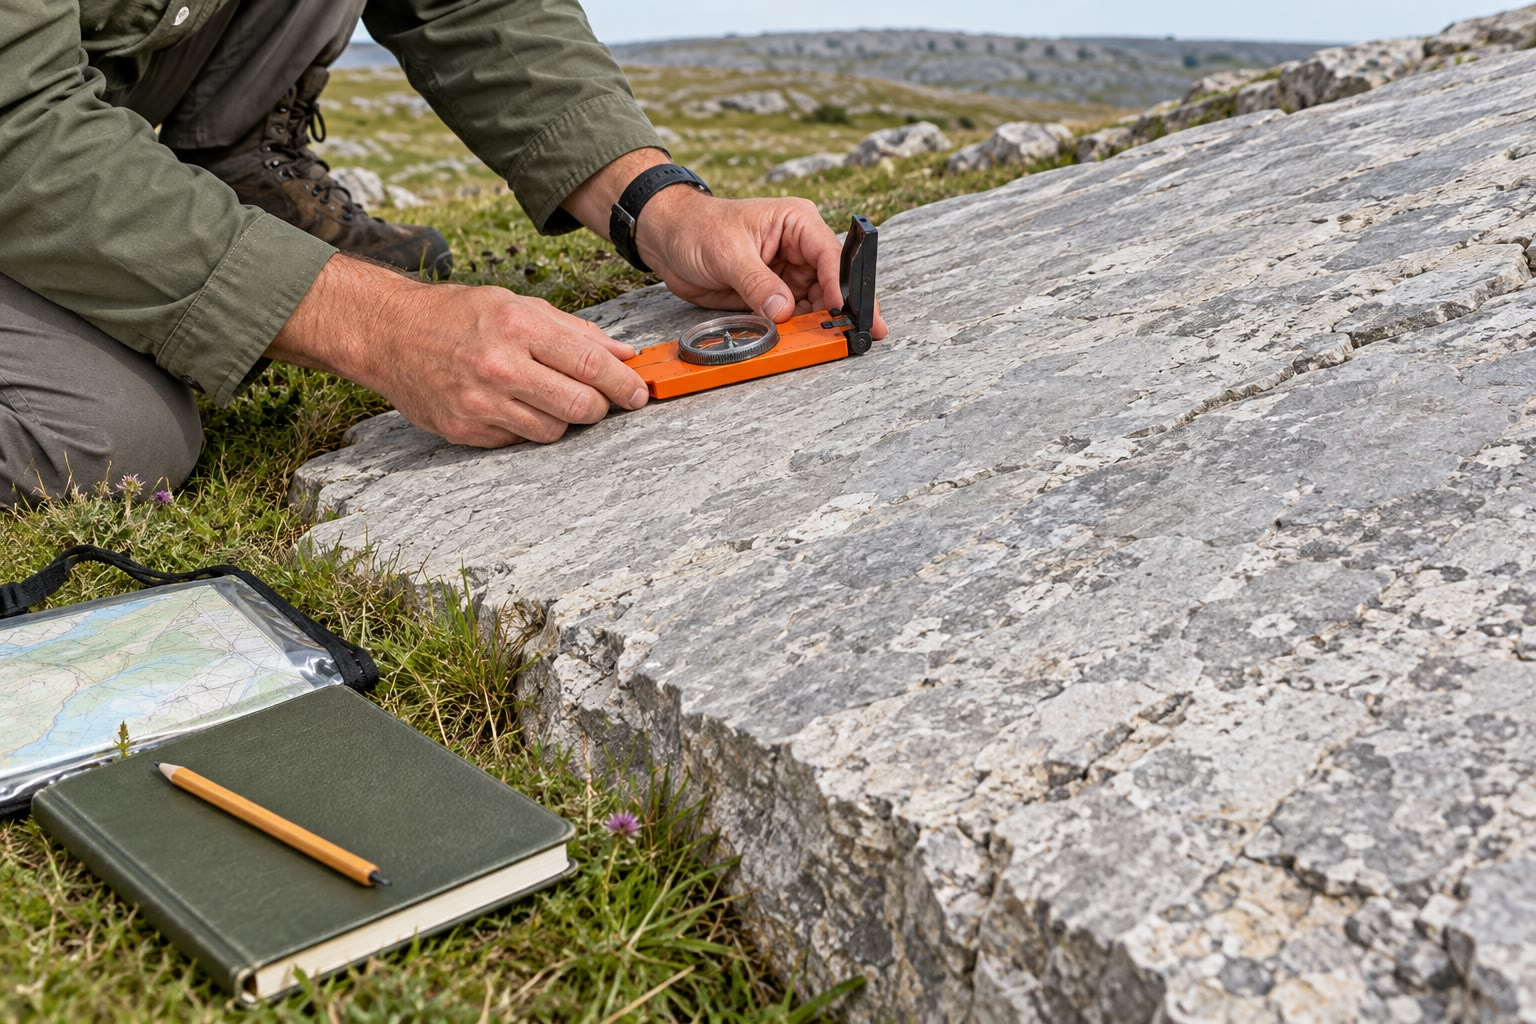
\includegraphics[width=0.6\linewidth]{images/book3/ai/b1-compass-clinometer.jpg}
\end{center}
\end{inthefield}

\begin{history}[The first geological map of a country]
% ledger: gsl:smith-1815, commons:smith-1815
The surveyor William Smith, who dug canals and drained land in England,
noticed that each layer of rock carried its own fossils, in an order that
was the same everywhere. Using the fossils to recognise the layers, he
followed them across the country for more than fifteen years. His map,
\emph{A Delineation of the Strata of England and Wales, with part of
Scotland}, dated 1 August 1815, is considered the first \omterm{def:b1:geological-maps:geological-map}{geological map} of a
complete country.
\begin{center}
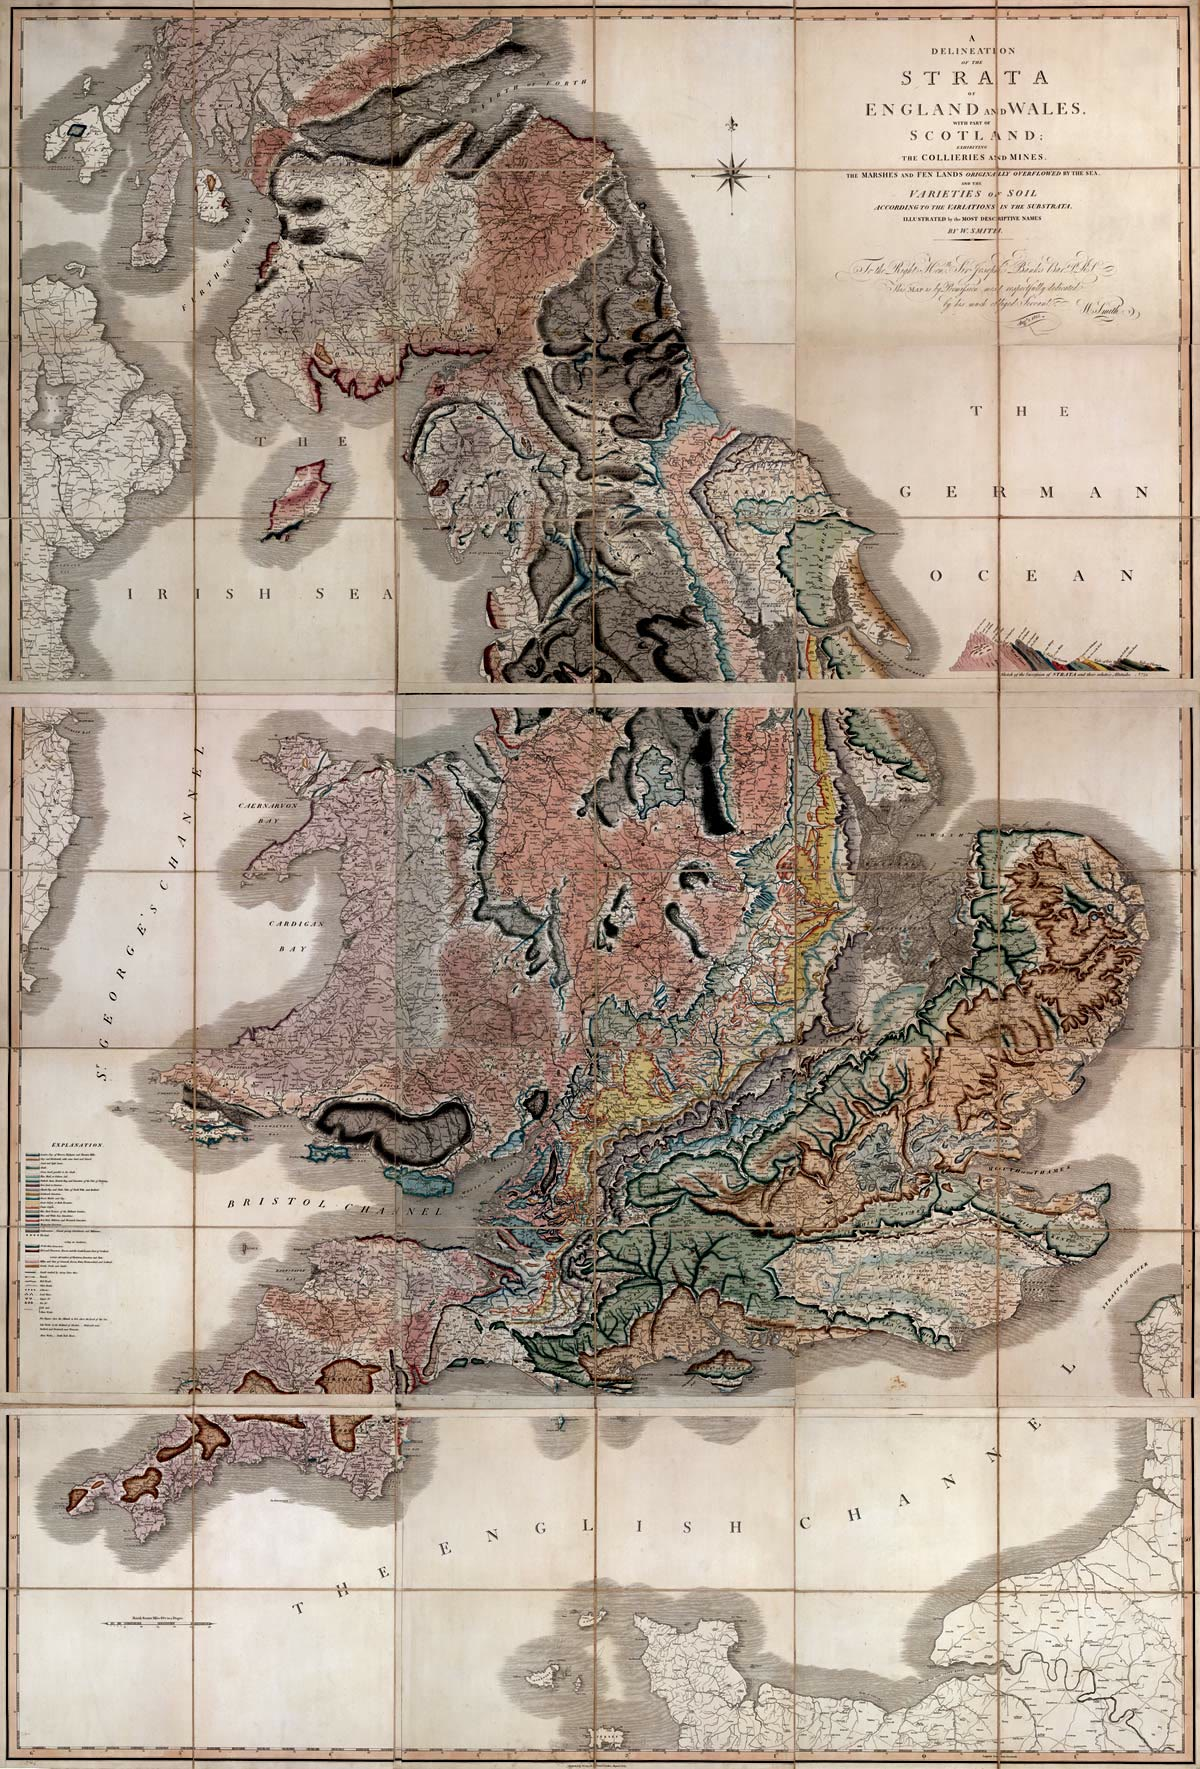
\includegraphics[width=0.36\linewidth]{images/book3/b1-smith-1815-map.jpg}

{\small William Smith's map of 1815 (public domain).}
\end{center}
\end{history}

\section{Exercises}

\begin{exercise}[$\star$]\label{exo:b1:geological-maps:1}
Define the \omterm{def:b1:geological-maps:attitude}{strike}, the \omterm{def:b1:geological-maps:attitude}{dip} and the \omterm{def:b1:geological-maps:attitude}{dip direction} of a plane. A bed has
\omterm{def:b1:geological-maps:attitude}{attitude} $135/40$: give its \omterm{def:b1:geological-maps:attitude}{strike} by the right-hand rule and draw its map
symbol.
\end{exercise}

\begin{exercise}[$\star$]\label{exo:b1:geological-maps:2}
Write the equation of the plane of \omterm{def:b1:geological-maps:attitude}{attitude} $090/30$ through the point
$(0, 0, 500)$, coordinates in metres. At what elevation is it at
$(1000, 0)$ and at $(0, 1000)$?
\end{exercise}

\begin{exercise}[$\star$]\label{exo:b1:geological-maps:3}
On a map, the trace of a contact follows the contour line \qty{350}{m}
exactly, over several kilometres of hills and valleys. What can you say
about the contact? And if its trace is a straight line across hills and
valleys?
\end{exercise}

\begin{exercise}[$\star$]\label{exo:b1:geological-maps:4}
On the map of the Varden Hills, which unit crops out in the core of the
\omterm{def:b1:geological-maps:fold}{anticline} along the river, and which unit occupies the core of the \omterm{def:b1:geological-maps:fold}{syncline}?
Explain why with the principle of superposition.
\end{exercise}

\begin{exercise}[$\star\star$]\label{exo:b1:geological-maps:5}
A contact is met at elevations $\qty{300}{m}$ at $(0, 0)$, $\qty{300}{m}$ at
$(1000, 0)$ and $\qty{200}{m}$ at $(0, 500)$ (metres, $x$ east, $y$ north).
Find its \omterm{def:b1:geological-maps:attitude}{strike}, \omterm{def:b1:geological-maps:attitude}{dip direction} and \omterm{def:b1:geological-maps:attitude}{dip}, first by reasoning on structure
contours, then with \cref{thm:b1:geological-maps:three-point}.
\end{exercise}

\begin{exercise}[$\star\star$]\label{exo:b1:geological-maps:6}
A valley floor descends northward at \qty{30}{m} per km. Which way does the
V of the \omterm{def:b1:geological-maps:geological-map}{outcrop} of a contact point if the contact (a) is horizontal; (b)
\omterm{def:b1:geological-maps:attitude}{dips} \ang{20} south; (c) \omterm{def:b1:geological-maps:attitude}{dips} \ang{1} north; (d) \omterm{def:b1:geological-maps:attitude}{dips} \ang{20} north? Justify
with \cref{thm:b1:geological-maps:v-rule}.
\end{exercise}

\begin{exercise}[$\star\star$]\label{exo:b1:geological-maps:7}
In the situation of the V-rule, a contact \omterm{def:b1:geological-maps:attitude}{dips} downstream with $a = 0.364$
(\ang{20}) and the valley floor descends with $s = 0.03$. A point on the
valley side is \qty{80}{m} higher than the floor. How far upstream of the
apex is the trace at that point?
\end{exercise}

\begin{exercise}[$\star\star$]\label{exo:b1:geological-maps:8}
The \omterm{def:b1:geological-maps:geological-map}{outcrops} of the Varden \omterm{def:b1:geological-maps:fold}{anticline} close around the north end of its core.
In which direction does the \omterm{def:b1:geological-maps:fold}{fold axis} plunge? Would the \omterm{def:b1:geological-maps:geological-map}{outcrops} of the
\omterm{def:b1:geological-maps:fold}{syncline} close to the north or to the south?
\end{exercise}

\begin{exercise}[$\star\star$]\label{exo:b1:geological-maps:9}
On the \omterm{def:b1:geological-maps:geological-map}{geological map}, along the fault, which side shows younger units at
the surface? Which block moved down? Check against the map symbol.
\end{exercise}

\begin{exercise}[$\star\star\star$]\label{exo:b1:geological-maps:10}
Show that two planes of \omterm{def:b1:geological-maps:attitude}{attitudes} $(\alpha_1, \delta_1)$ and
$(\alpha_2, \delta_2)$ intersect along a line parallel to
$\vec n_1 \times \vec n_2$, where $\vec n_i = (\tan\delta_i\sin\alpha_i,
\tan\delta_i\cos\alpha_i, 1)$. Apply it to the planes $090/30$ and $270/30$:
what is the line, and what kind of \omterm{def:b1:geological-maps:fold}{fold} do the two planes make?
\end{exercise}

\begin{exercise}[$\star\star\star$]\label{exo:b1:geological-maps:11}
A vertical dyke \omterm{def:b1:geological-maps:attitude}{strikes} \ang{045} and crops out at the origin, on a valley
floor at elevation \qty{0}{m}. Where can its trace lie on a hill at
\qty{300}{m}? A second dyke has the same \omterm{def:b1:geological-maps:attitude}{strike}, \omterm{def:b1:geological-maps:attitude}{dips} \ang{60} to the
south-east and also crops out at the origin. How far from the origin, and in
which direction, does its trace lie on ground at \qty{300}{m}, measured
perpendicular to the \omterm{def:b1:geological-maps:attitude}{strike}?
\end{exercise}

\begin{exercise}[$\star\star\star$]\label{exo:b1:geological-maps:12}
In a \omterm{def:b1:geological-maps:dem}{digital elevation model} with a \qty{100}{m} grid, the ground at
$(x, y)$ and at $(x + 100, y)$ is at 420 and \qty{405}{m}, and at
$(x, y + 100)$ at \qty{412}{m}. Treating the ground in that cell as a plane,
compute its slope (in degrees) and the \omterm{def:b1:spherical-astronomy:horizontal}{azimuth} toward which it faces
(down-slope direction).
\end{exercise}

\section{Problem: Solving the Varden Hills}

\begin{problem}[{Weekend problem --- from boreholes and a map to the fold axis,
the fault and the history of a region}]
\label{pb:b1:geological-maps:1}
% all data computed in figdata/bachelor-1/varden_maps.py from the region's
% model (figdata/shared/region.py); invented region: exercise data, no ledger
A company drilling for water in the Varden Hills records where its boreholes
meet the base of the limestone; its geologists also locate the fault where it
crosses the ground. Coordinates are in metres east and north of the map's
south-west corner; elevations in metres above sea level. Part I uses the
coloured \omterm{def:b1:geological-maps:geological-map}{geological map} of \cref{sec:b1:geological-maps:cut}.

\medskip
\noindent\textbf{Part I --- Reading the map.}
\begin{enumerate}
  \item List the units of the region from the oldest to the youngest.
  \item Which units does the river cut through, from west to east?
  \item Which unit occupies the core of the \omterm{def:b1:geological-maps:fold}{fold} near $x = \qty{3.5}{km}$?
        What kind of \omterm{def:b1:geological-maps:fold}{fold} is it?
  \item Which unit occupies the core of the \omterm{def:b1:geological-maps:fold}{fold} near $x = \qty{7.5}{km}$?
        What kind of \omterm{def:b1:geological-maps:fold}{fold} is it?
  \item Why are the schist and the granite visible only near the river, in
        the core of the first \omterm{def:b1:geological-maps:fold}{fold}?
  \item What kind of contact separates the sandstone from the granite?
        Justify from the map.
\end{enumerate}

\medskip
\noindent The boreholes (depth $d$ to the base of the limestone, ground
elevation $z_g$) and the three points F1--F3 where the fault crosses the
top of the bedrock (F2, in the valley, lies under the thin alluvium, which
the fault does not cut):

\begin{omfigure}
\begin{minipage}[c]{0.42\linewidth}
\centering\small
\begin{tabular}{lrrrr}
\hline
 & east & north & $z_g$ & $d$ \\
\hline
E1 & 4000 & 6000 & 435 & 261 \\
E2 & 4600 & 7200 & 432 & 428 \\
E3 & 5100 & 6400 & 512 & 586 \\
W1 & 1500 & 6000 & 524 & 669 \\
W2 & 2200 & 7200 & 421 & 459 \\
W3 & 2600 & 5400 & 319 & 209 \\
\hline
 & east & north & $z_g$ & \\
\hline
F1 & 4197 & 1000 & 405 & \\
F2 & 5824 & 3500 & 129 & \\
F3 & 7321 & 6500 & 482 & \\
\hline
\end{tabular}
\end{minipage}\hfill
\begin{minipage}[c]{0.56\linewidth}
\centering
\begin{tikzpicture}
\begin{axis}[axis equal image, xmin=0, xmax=10, ymin=0, ymax=8, width=\linewidth,
  tick label style={font=\scriptsize}, xlabel={east (km)}, ylabel={north (km)},
  label style={font=\footnotesize}]
\addplot[fill=black!8, draw=black!50, line width=0.3pt, even odd rule] table {figdata/out/shared-region-unit-schist.dat};
\addplot[fill=black!8, draw=black!50, line width=0.3pt, even odd rule] table {figdata/out/shared-region-unit-granite.dat};
\addplot[fill=icsTriassic!20, draw=black!50, line width=0.3pt, even odd rule] table {figdata/out/shared-region-unit-sandstone.dat};
\addplot[fill=icsJurassic!25, draw=black!50, line width=0.3pt, even odd rule] table {figdata/out/shared-region-unit-limestone.dat};
\addplot[fill=icsJurassic!8, draw=black!50, line width=0.3pt, even odd rule] table {figdata/out/shared-region-unit-shale.dat};
\addplot[fill=icsCretaceous!20, draw=black!50, line width=0.3pt, even odd rule] table {figdata/out/shared-region-unit-chalk.dat};
\addplot[fault] table {figdata/out/shared-region-fault.dat};
\addplot[fill=omLithAlluv, draw=black!50, line width=0.3pt, even odd rule] table {figdata/out/shared-region-unit-alluvium.dat};
\addplot[river] table {figdata/out/shared-region-river.dat};
\addplot[only marks, mark=*, mark size=1.6pt] table[x=x_km, y=y_km] {figdata/out/bachelor-1-varden_maps-boreholes.dat};
\addplot[only marks, mark=square*, mark size=1.5pt, omThm] table[x=x_km, y=y_km] {figdata/out/bachelor-1-varden_maps-fault.dat};
\begin{scope}[every node/.style={font=\scriptsize\bfseries, inner sep=1.5pt, fill=white, fill opacity=0.8, text opacity=1}]
  \node[above right] at (axis cs:4,6) {E1};
  \node[above] at (axis cs:4.6,7.2) {E2};
  \node[right] at (axis cs:5.1,6.4) {E3};
  \node[above left] at (axis cs:1.5,6) {W1};
  \node[above] at (axis cs:2.2,7.2) {W2};
  \node[left] at (axis cs:2.6,5.4) {W3};
  \node[left, text=omThm] at (axis cs:4.197,1) {F1};
  \node[left, text=omThm] at (axis cs:5.824,3.5) {F2};
  \node[left, text=omThm] at (axis cs:7.321,6.5) {F3};
\end{scope}
\end{axis}
\end{tikzpicture}
\end{minipage}
\end{omfigure}

\medskip
\noindent\textbf{Part II --- The east limb.}
\begin{enumerate}[resume]
  \item Compute the elevation of the base of the limestone in E1, E2 and E3.
  \item Write the vectors $\overrightarrow{E_1E_2}$ and
        $\overrightarrow{E_1E_3}$.
  \item Compute their cross product and orient it upward.
  \item Deduce the \omterm{def:b1:geological-maps:attitude}{dip} of the base of the limestone on the east limb.
  \item Deduce its \omterm{def:b1:geological-maps:attitude}{dip direction}, then its \omterm{def:b1:geological-maps:attitude}{strike} by the right-hand rule.
  \item Is the result consistent with the strike-and-dip symbol of the east
        limb on the map?
\end{enumerate}

\medskip
\noindent\textbf{Part III --- The fold.}
\begin{enumerate}[resume]
  \item Compute the elevations of the base of the limestone in W1, W2 and
        W3.
  \item Compute an upward normal $\vec n_W$ to the base of the limestone on
        the west limb.
  \item Deduce the \omterm{def:b1:geological-maps:attitude}{attitude} of the west limb.
  \item Compute a direction of the intersection of the two limbs, the \omterm{def:b1:geological-maps:fold}{fold
        axis}, as $\vec n_E \times \vec n_W$ (with $\vec n_E$ from question 9).
  \item Give the trend (the \omterm{def:b1:spherical-astronomy:horizontal}{azimuth} of the axis's horizontal projection,
        taken downward) and the plunge (its angle below the horizontal) of
        the \omterm{def:b1:geological-maps:fold}{fold axis}.
  \item The base of the sandstone lies on the axis at \qty{230}{m} where the
        river crosses it, near $y = \qty{4}{km}$. How much lower is it on the
        axis \qty{8}{km} farther north? Is this consistent with question 3 of
        Part I and with the closure of the \omterm{def:b1:geological-maps:geological-map}{outcrops}?
\end{enumerate}

\medskip
\noindent\textbf{Part IV --- The fault and the history.}
\begin{enumerate}[resume]
  \item From F1, F2 and F3, compute the \omterm{def:b1:geological-maps:attitude}{attitude} of the fault.
  \item Along the fault, the units at the surface on the east-south-east side
        are younger than those opposite them. Which block moved down? Is the
        fault normal or reverse?
  \item The straight line from F1 to F3 passes about \qty{200}{m} west of F2.
        Why does the trace of the fault bend toward the east-south-east where
        it crosses the river valley, at F2?
  \item Put in order: folding; deposition of the chalk; faulting; intrusion
        of the granite; erosion before the sandstone; deposition of the
        alluvium.
  \item The chalk is 90 million years old and is folded; the alluvium was
        laid down in the last 2.58 million years and is not faulted. Between
        what ages did the folding and the faulting take place?
  \item To reach the fault at \qty{1000}{m} below sea level beneath F1, how
        far from F1, and in which direction, must a vertical well be drilled?
\end{enumerate}
\end{problem}
